%!TEX root = ../main.tex
\myChapter{Richiami di base}
In questo capitolo verranno richiamate alcune definizioni base che risulteranno fondamentali per la comprensione delle sezioni successive. Cominciando dalle basi di probabilità \cite{B12} si arriverà a formulare le definizioni dei principali modelli utilizzati: \acf{dtmc} e \acf{mdp} \cite{KNP11}.

\begin{mtdef}[Esperimento casuale $\mathcal{C}$]
	Per esperimento casuale si intende un qualsiasi avvenimento, provocato più o meno direttamente dall'uomo, suscettibile di manifestarsi secondo una pluralità di \emph{eventi elementari}.
\end{mtdef}

\begin{mtdef}[Spazio fondamentale $\Omega$]
	Lo \emph{spazio fondamentale} $\Omega$ di $\mathcal{C}$ è l'insieme di tutti i suoi eventi elementari. Indichiamo tali eventi elementari come gli elementi $\omega \in \Omega$.
\end{mtdef}

\begin{mtdef}[Eventi casuali $\mathcal{E}$]
	Un \emph{evento casuale} $A \in \mathcal{E}$ è una proposizione relativa all'esito di un evento casuale $\mathcal{C}$ che, prima del compimento di $\mathcal{C}$, è in qualche modo incerto.
\end{mtdef}

\begin{mtobs}
	$\mathcal{E}$ contiene sottoinsiemi di $\Omega$
	$$ A \in \mathcal{E} \Rightarrow A \subseteq \Omega $$
\end{mtobs}

\begin{mtdef}[$\sigma$-algebra]
	Sia $\Omega$ lo spazio fondamentale dell'evento casuale $\mathcal{C}$. $\mathcal{F} \subseteq 2^\Omega$ è una $\sigma$-algebra se e solo se
	\begin{itemize}
		\item $\Omega \in \mathcal{F}$,
		\item $A \in \mathcal{F} \Rightarrow \overline{A} \in \mathcal{F}$,
		\item $\bigwedge_{i=1}^{\infty} A_i \in \mathcal{F} \Rightarrow \bigcup_{i=1}^\infty A_i \in \mathcal{F}$ \\ oppure $A_i \in \mathcal{F} (i \in I) \Rightarrow \bigcup_{i \in I} \in \mathcal{F} \wedge \bigcap_{i \in I} A_i \in \mathcal{F}$.
	\end{itemize}
\end{mtdef}

Gli elementi di una $\sigma$-algebra sono chiamati \emph{insiemi misurabili}. Chiamiamo \emph{spazio misurabile} uno spazio fondamentale su cui è definita una $\sigma$-algebra e quindi lo identifichiamo con la coppia $(\Omega, \mathcal{F})$.

\begin{mtdef}[Insieme dei rettangoli]
	Sia $\Omega=\mathbb{R}$, l'\emph{insieme dei rettangoli} è definito come $$ \mathcal{I} = \{(a,b] \sep a,b\in \mathbb{R} \cup \{-\infty,\infty\}\}. $$
\end{mtdef}

\begin{mtdef}[Insieme di Borel]
	Un \emph{insieme di Borel} $\mathcal{B}(\mathbb{R})$ è la più piccola $\sigma$-algebra che contiene l'insieme dei rettangoli $\mathcal{I}$.
\end{mtdef}

\begin{mtdef}[Spazio di Borel]
	Uno \emph{spazio di Borel} su $\mathbb{R}$ è lo spazio misurabile $(\mathbb{R},\mathcal{B}(\mathbb{R}))$.
\end{mtdef}

\begin{mtdef}[Assiomi di Kolmogoroff]
	Dato lo spazio misurabile $(\Omega,\mathcal{F})$, una \emph{misura di probabilità} su di esso è una funzione $\mathbb{P} : \mathcal{F} \rightarrow \mathbb{R}_{\geq 0}$ tale che
	\begin{equation*}
		\mathbb{P}(\emptyset) = 0
	\end{equation*}
	\begin{equation*}
		\mathbb{P}(\Omega) = 1
	\end{equation*}
	e, per qualsiasi famiglia $\{A_i \sep A_i \in \mathcal{F}, i \in \mathbb{N}\}$ tale che $k \neq h \Rightarrow A_k \cap A_h = \emptyset$, vale:
	\begin{equation*}
		 \mathbb{P}\left(\bigcup_{i=1}^\infty A_i\right) = \sum_{i=1}^\infty \mathbb{P}\left(A_i\right)
	\end{equation*}
\end{mtdef}

Chiamiamo \emph{spazio di probabilità} dell'esperimento casuale $\mathcal{C}$ la tripla $(\Omega, \mathcal{F}, \mathbb{P})$, dove $\Omega$ è lo spazio fondamentale, $(\Omega, \mathcal{F})$ lo spazio misurabile e $\mathbb{P}$ la misura di probabilità su $\mathcal{F}$.
Se esiste l'insieme numerabile $A \subseteq \Omega$ tale che $\sum_{a \in A} \mathbb{P}\{a\} = 1$ allora diciamo che $\mathbb{P}$ è una \emph{misura di probabilità discreta} e $(\Omega, \mathcal{F}, \mathbb{P})$ è uno \emph{spazio di probabilità discreto}.

\begin{mtpro}[Proprietà di $\mathbb{P}$]
	Dato lo spazio di probabilità $(\Omega, \mathcal{F}, \mathbb{P})$:
	\begin{enumerate}
		\item $\forall A \in \mathcal{F}: \mathbb{P}A + \mathbb{P}\overline{A} = 1$,
		\item $\forall A,B \in \mathcal{F} : A \subseteq B \Rightarrow \mathbb{P} A \leq \mathbb{P} B$,
		\item $\forall A \in \mathcal{F} : \mathbb{P} A \leq 1$,
		\item $\forall A, B \in \mathcal{F} : \mathbb{P}(A\cup B) \geq \max\{\mathbb{P}A, \mathbb{P}B\}$,
		\item $\forall A, B \in \mathcal{F} : \mathbb{P}{A\cap B} \leq \min \{\mathbb{P}A,\mathbb{P}B\}$,
		\item $\forall A,B \in \mathcal{F} : \mathbb{P}(A\cup B) = \mathbb{P}A + \mathbb{P}B - \mathbb{P}(A\cap B)$,
		\item $\forall A,B \in \mathcal{F} : A \subseteq B \Rightarrow \mathbb{P}(B \backslash A) = \mathbb{P}B - \mathbb{P}A$,
		\item $\forall A_i \in \mathcal{F} : \mathbb{P}\left( \bigcup_{i=0}^\infty A_i \right) \leq \sum_{i=0}^\infty \mathbb{P} A_i$.
	\end{enumerate}
\end{mtpro}

\begin{mtdef}[Probabilità condizionale]
	Dato lo spazio di probabilità $(\Omega, \mathcal{F}, \mathbb{P})$ e $A,B \in \mathcal{F}$ tali che $\mathbb{P}B > 0$ si definisce \emph{probabilità condizionale}
	$$ \mathbb{P}(A | B) = \frac{\mathbb{P}(A \cap B)}{\mathbb{P}B} $$
	o alternativamente
	$$ \mathbb{P}(A | B) \cdot \mathbb{P}B = \mathbb{P}(A \cap B) = \mathbb{P}(B | A) \cdot \mathbb{P}A $$
\end{mtdef}

\begin{mtdef}[Eventi stocasticamente indipendenti]
	Due eventi $A$ e $B$ sono \emph{stocasticamente indipendenti} se e solo se
	$$ \mathbb{P}(A\cap B) = \mathbb{P}A \cdot \mathbb{P}B$$
\end{mtdef}

\begin{mtpro}[Proprietà di eventi stocasticamente indipendenti]
	Se $A$ e $B$ sono eventi stocasticamente indipendenti allora valgono le seguenti proprietà:
	\begin{enumerate}
		\item $\overline{A}$ e $B$ sono stocasticamente indipendenti,
		\item $A$ e $\overline{B}$ sono stocasticamente indipendenti,
		\item $\overline{A}$ e $\overline{B}$ sono stocasticamente indipendenti,
		\item $\mathbb{P}(A\cup B) = 1 - \mathbb{P}\overline{A} \cdot \mathbb{P}B$.
	\end{enumerate}
\end{mtpro}

\section{Variabili casuali}

Una variabile casuale è definita da una funzione che assegna un valore a ogni elemento dello spazio fondamentale $\Omega$.

\begin{mtdef}[Funzione misurabile]
	Dati gli spazi misurabili $(\Omega_1,\mathcal{F}_1)$ e $(\Omega_2,\mathcal{F}_2)$, $f:\Omega_1 \rightarrow \Omega_2$ è una \emph{funzione misurabile} se e solo se
	$$ \forall A \in \mathcal{F}_2 : f^{orig}(A) \triangleq \{\omega \in \Omega_1 \sep f(\omega) \in A \} \in \mathcal{F}_1 $$
\end{mtdef}

\begin{mtdef}[Variabile casuale]
	Una \emph{variabile casuale} è definita da una funzione misurabile
	$$ X : \Omega \rightarrow \mathbb{R} $$
	dove $(\mathbb{R},\mathcal{B}(\mathbb{R}))$ è lo spazio di Borel su $\mathbb{R}$.
\end{mtdef}

\begin{mtpro}
	Dato $(\Omega_1,\mathcal{F}_1,\mathbb{P})$ spazio di probabilità, $(\Omega_2,\mathcal{F}_2)$ spazio misurabile e $f:\Omega_1 \rightarrow \Omega_2$ funzione misurabile, allora:
	$$ (\Omega_2, \mathcal{F}_2, \mathbb{P} \circ f^{orig}) $$
	è uno spazio di probabilità.
\end{mtpro}

\section{Processi stocastici}

\begin{mtdef}[Processo stocastico]
	Un \emph{processo stocastico} è una famiglia $T$-indicizzata di variabili casuali, dove $T \subseteq \mathbb{R}^+$ è lo spazio della variabile temporale
	$$ \{X_i \sep i \in T\} $$
\end{mtdef}

L'insieme $T$ può essere considerato sia continuo che discreto e, a seconda del caso, si può formulare nelle due seguenti definizioni:

\begin{mtdef}[Processo stocastico discreto]
	Un \emph{processo stocastico discreto} è un processo stocastico con $T = \mathbb{N}$
	$$ \{X_n \sep n \in \mathbb{N}\} $$
\end{mtdef}

\begin{mtdef}[Processo stocastico continuo]
	Un \emph{processo stocastico continuo} è un processo stocastico con $T = \mathbb{R}$
	$$ \{X_t \sep t \in \mathbb{R}\} $$
\end{mtdef}

\section{Discrete-Time Markov Chains}

Le \ac{dtmc} sono processi stocastici discreti $\{X_n \sep n \in \mathbb{N}\}$ aventi uno spazio degli stati discreto e che godono della proprietà di \emph{assenza di memoria} di Markov
$$ \mathbb{P}\{X_{n} = i_{n}\sep X_{n-1} = i_{n-1}, \dots, X_0=i_0 \} = \mathbb{P}\{X_{n} = i_{n}\sep X_{n-1} = i_{n-1}\}. $$
Definiamo una \ac{dtmc} come segue
\begin{mtdef}[\ac{dtmc}]
	Una \ac{dtmc} è una tupla $\mathcal{D} = (S,\overline{s},\mathbb{P})$ dove:
	\begin{itemize}
		\item $S$ è un insieme finito di \emph{stati};
		\item $\overline{s} \in S$ è lo \emph{stato iniziale};
		\item $\mathbb{P} : S \times S \rightarrow [0,1]$ è la \emph{matrice di probabilità delle transizioni}, tale che:
		$$ \sum_{s' \in S} \mathbb{P}(s,s') = 1$$
		per ogni stato $s \in S$.
	\end{itemize}
\end{mtdef}

\begin{mtdef}[\ac{dtmc} path]
	Un cammino $\pi$ di una \ac{dtmc} $\mathcal{D} = (S,\overline{s}, \mathbb{P})$ che comincia da $s \in S$ è una sequenza non vuota $s_0, s_1, s_2, \dots$ di stati tali che:
	\begin{enumerate}
		\item $s = s_0$
		\item $\forall\ i : \mathbb{P}(s_i, s_{i+1}) > 0$
	\end{enumerate} 
\end{mtdef}

\begin{mtobs}
	Un cammino $\pi$ di una \ac{dtmc} può essere finito o infinito.
\end{mtobs}

\begin{mtdef}[\ac{dtmc} path up to $n$]
	Sia $\pi$ un cammino, il cammino \emph{up to $n$}, o $\pi \uparrow n$, è il prefisso $s_0, \dots, s_n$ di $\pi$.
\end{mtdef}

\begin{mtdef}[\ac{dtmc} paths]
	$Paths_{s_0}^{\mathcal{D}}$ o $Paths(\mathcal{D}, s_0)$, è l'insieme di tutti i cammini di una \ac{dtmc} $\mathcal{D}$ che cominciano in $s_0$.
\end{mtdef}

Utilizziamo inoltre le seguenti notazioni riguardanti i cammini su \ac{dtmc}:
\begin{itemize}
	\item $\pi(i)$ indica l'$i$-esimo stato del cammino $\pi$,
	\item $|\pi|$ indica la lunghezza del cammino $\pi$,
	\item $last(\pi)$ indica l'ultimo stato del cammino finito $\pi$ e
	\item $Paths^{fin}_s$ indica l'insieme di tutti i cammini finiti che cominciano in $s$.
\end{itemize}

Illustriamo con un esempio la struttura appena definita: in figura \ref{fig:dtmc:esempio} viene raffigurata con una notazione grafica una \ac{dtmc} a quattro stati. Nella rappresentazione gli stati sono indicati come cerchi e le transizioni come frecce etichettate con la probabilità associata. Lo stato iniziale viene indicato con una freccia entrante.
\begin{figure}[htb]
	\begin{center}
		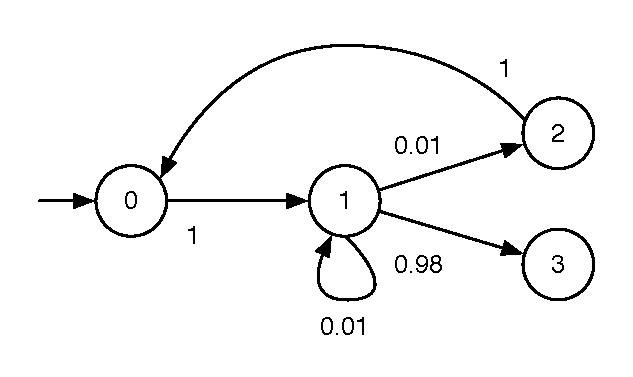
\includegraphics[width=.5\textwidth]{Images/exdtmc}
	\end{center}
	\caption{Rappresentazione grafica di una \acs{dtmc} a quattro stati}
	\label{fig:dtmc:esempio}
\end{figure}
La matrice di probabilità associata a questa \ac{dtmc} avrà la seguente forma:
$$
\mathbb{P} = 
\left(
\begin{array}{cccc}
	0&1&0&0 \\
	0&0.01&0.01&0.98 \\
	1&0&0&0 \\
	0&0&0&1 \\
\end{array}
\right)
.
$$
L'esempio può rappresentare un processo che tenta di spedire un messaggio: dallo stato iniziale $0$ si entra nello stato $1$ dove con probabilità $0.01$ si aspetta l'istante successivo, con probabilità $0.98$ si consegna il messaggo con successo e con probabilità $0.01$ la consegna fallisce. In caso di fallimento il processo ricomincia dallo stato iniziale mentre in caso di successo si entra permanentemente nello stato $3$.

Definiamo la misura di probabilità di un singolo cammino.
\begin{mtdef}
Sia $\pi_{fin} \in Paths^{fin}_s$ un qualsiasi cammino finito, la probabilità di un  cammino finito si definisce come segue
$$
	\mathbb{P}_s(\pi_{fin}) \triangleq \left\{
	\begin{array}{ll}
		1 & \mbox{se } n=0 \\
		\mathbb{P}(\pi(0),\pi(1))\dots\mathbb{P}(\pi(n-1),\pi(n)) & \mbox{altrimenti} \\
	\end{array}
	\right.
$$
dove $n = |\pi_{fin}|$.
\end{mtdef}

\begin{mtdef}[Insieme dei cilindri]
	Sia $n \in \mathbb{N}_0$ e $\mathcal{D}$ una \ac{dtmc}, definiamo un \emph{insieme dei cilindri} come
$$ 
C(\pi_{fin}) \triangleq \{\pi \in Paths^\mathcal{D}_s \sep \pi_{fin} \mbox{ è un prefisso di } \pi \} 
$$
\end{mtdef}
L'insieme dei cilindri quindi rappresenta tutti i cammini che hanno come prefisso comune il cammino finito specificato. Definiamo poi la misura di probabilità di un singolo cammino

Forniamo infine la misura di probabilità di un insieme di cammini di una \ac{dtmc}
\begin{mtdef}
	Sia $\pi_{fin} \in Paths^{fin}_s$ un qualsiasi cammino finito, la probabilità di un insieme di cammini è definita come segue
$$ Prob_s(C(\pi_{fin})) = \mathbb{P}_s(\pi_{fin}). $$
\end{mtdef}

Di seguito riportiamo alcuni esempi di probabilità su insiemi di cammini della \ac{dtmc} di figura \ref{fig:dtmc:esempio}:
$$
\begin{array}{l}
	Prob_0(C(0,1,1,1)) = 1 \cdot 0.01 \cdot 0.01 = 0.00001 \\
	Prob_0(C(0,1,1,2)) = 1 \cdot 0.01 \cdot 0.01 = 0.00001 \\
	Prob_0(C(0,1,1,3)) = 1 \cdot 0.01 \cdot 0.98 = 0.00098 \\
	Prob_0(C(0,1,2,0)) = 1 \cdot 0.01 \cdot 1 = 0.01 \\
	Prob_0(C(0,1,3,3)) = 1 \cdot 0.98 \cdot 1 = 0.98 \\
\end{array}
$$

\section{Markov Decision Processes}

Le \ac{mdp} estendono le \ac{dtmc} aggiungendo la possibilità di esprimere \emph{nondeterminismo}. Il nondeterminismo è un meccanismo di astrazione che permette di nascondere qualsiasi aspetto quantitativo che caratterizza una scelta, come le probabilità. Non si può quindi fare alcuna assunzione su come verrà presa una scelta deterministica ma sono note le scelte possibili.

\begin{mtdef}
	Un \ac{mdp} è una tupla $\mathcal{M} = (S, \overline{s}, Act, Steps)$ dove:
	\begin{itemize}
		\item $S$ è un insieme finito di \emph{stati};
		\item $\overline{s} \in S$ è lo \emph{stato iniziale};
		\item $Act$ è un insieme di \emph{azioni};
		\item $Steps: S \rightarrow 2^{Act \times Dist(S)}$ è la \emph{funzione di transizione probabilistica}.
	\end{itemize}
\end{mtdef}

\begin{mtdef}[\ac{mdp} path]
	Un cammino $\pi$ di una \ac{mdp} $\mathcal{M} = (S,\overline{s},Act,Steps)$ che comincia da $s_0$ è una sequenza non vuota $$s_0, a_1, \mu_1, s_1, a_2, \mu_2, s_3, \dots$$ dove $s_i \in S$, $(a_{i+1},\mu_{i+1})\in Steps(s_i)$ e $\mu_{i+1}(s_{i+1}) > 0$ per ogni $i\geq 0$.
\end{mtdef}

\begin{mtobs}
	Un cammino $\pi$ di una \ac{mdp} può essere finito o infinito.
\end{mtobs}

\begin{mtdef}[\ac{mdp} path up to $n$]
	Sia $\pi$ un cammino, il cammino \emph{up to $n$}, o $\pi \uparrow n$, è il prefisso $s_0, \dots, s_n$ di $\pi$.
\end{mtdef}

\begin{mtdef}[\ac{mdp} paths]
	$paths_{s_0}^{\mathcal{M}}$ o $paths(\mathcal{M}, s_0)$, è l'insieme di tutti i cammini della \ac{mdp} $\mathcal{M}$ che cominciano in $s_0$.
\end{mtdef}

Analogamente alle \ac{dtmc}, anche per le \ac{mdp} utilizziamo le seguenti notazioni:
\begin{itemize}
	\item $\pi(i)$ indica l'$i$-esimo stato del cammino $\pi$,
	\item $|\pi|$ indica la lunghezza del cammino $\pi$,
	\item $last(\pi)$ indica l'ultimo stato del cammino finito $\pi$ e
	\item $Paths^{fin}_s$ indica l'insieme di tutti i cammini finiti che iniziano in $s$.
\end{itemize}

Riportiamo un esempio di \ac{mdp} in figura \ref{fig:mdp:esempio}. La rappresentazione grafica estende quella utilizzata nell'esempio di \ac{dtmc} in figura \ref{fig:mdp:esempio} aggiungendo delle etichette che riportano il nome dell'azione eseguita dalle transizioni. Nello stato iniziale $0$ ci si muove sempre nello stato $1$ compiendo l'azione $a$ dove abbiamo una scelta nondeterministica tra le azioni $b$ e $c$. Scegliendo $b$ avremo una probabilità $0.7$ di tornare allo stato iniziale e $0.3$ di restare nello stato $1$. Se invece viene scelta l'azione $c$ gli stati di arrivo $2$ e $3$ avranno ciascuno probabilità $0.5$.
\begin{figure}[htb]
	\begin{center}
		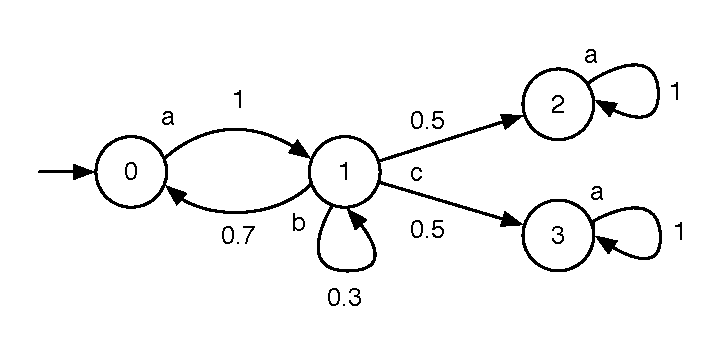
\includegraphics[width=.5\textwidth]{Images/exmdp}
	\end{center}
	\caption{Rappresentazione grafica di una \acs{mdp} a quattro stati}
	\label{fig:mdp:esempio}
\end{figure}

\begin{mtdef}[Scheduler]
	Uno \emph{scheduler} $\Sigma$ di una \ac{mdp} $\mathcal{M}$ è una funzione che mappa tutti gli elementi di $\pi_{fin}$ di $\mathcal{M}$ in un elemento dell'insieme $Steps(last(\pi_{fin}))$ indicato con $S(\pi_{fin})$. Con $Scheduler_{\mathcal{M}}$ denotiamo l'insieme di tutti i possibili scheduler di $\mathcal{M}$ e, per ogni scheduler $\Sigma$, indichiamo con $path_s^\Sigma$ il sotto insieme di $path_s$ che corrisponde a $\Sigma$.
\end{mtdef}

Facendo riferimento all'esempio di figura \ref{fig:mdp:esempio} descriviamo dei possibili scheduler $\Sigma_1$ e $\Sigma_2$ di quella \ac{mdp}. Useremo le notazioni $\mu_b$ e $\mu_c$ per rappresentare rispettivamente le distribuzioni derivanti dalla scelta delle azioni $b$ e $c$ presenti nello stato $1$.
\begin{itemize}
	\item $\Sigma_1 : \Sigma_1(0,a,1) = \mu_c$
	\item $\Sigma_2 : \Sigma_2(0,a,1) = \mu_b, \Sigma_2(0,a,1,b,1) = \mu_c, \Sigma_2(0,a,1,b,0,a,1) = \mu_c$
\end{itemize}
Entrambi gli scheduler risolvono tutte le scelte nondeterministiche che si possono trovare durante l'esecuzione riducendo la \ac{mdp} a una \ac{dtmc}. Una volta giunti agli stati $2$ e $3$, infatti, non sarà più possibile tornare agli stati precedenti o eseguire qualsiasi tipo di scelta.

Formalizziamo il passaggio da una \ac{mdp} $\mathcal{M} = (S,\overline{s},Act,Steps)$ alla \ac{dtmc} $\mathcal{D}^{\Sigma} = (S^\Sigma,\overline{s}^\Sigma,\mathbb{P}^\Sigma) $ applicando lo scheduler $\Sigma$. Il comportamento di uno stato $s \in S$ può essere descritto infatti con la  \ac{dtmc} a stati infiniti la cui struttura dipenderà da quella della \ac{mdp} nel seguente modo:
\begin{itemize}
	\item $S^\Sigma = Paths_s^{fin}$,
	\item $\overline{s}^\Sigma = s$
	\item per due cammini finiti $\pi,\pi' \in S^\Sigma$:
	$$
	\mathbb{P}^\Sigma (\pi,\pi') = \left\{
	\begin{array}{ll}
		\mu(s') & \mbox{se } \pi' \mbox{ è della forma } \pi,\Sigma(\pi),s' \mbox{ con } \Sigma(\pi) = (a,\mu)\\
		0 & \mbox{altrimenti}
	\end{array}
	\right.
	$$
\end{itemize}
In figura \ref{fig:mdp:scheduler} viene riportata la \ac{dtmc} $\mathcal{D}^{\Sigma_1}$ ottenuta dall'esempio di scheduler $\Sigma_1$.
\begin{figure}[htb]
	\begin{center}
		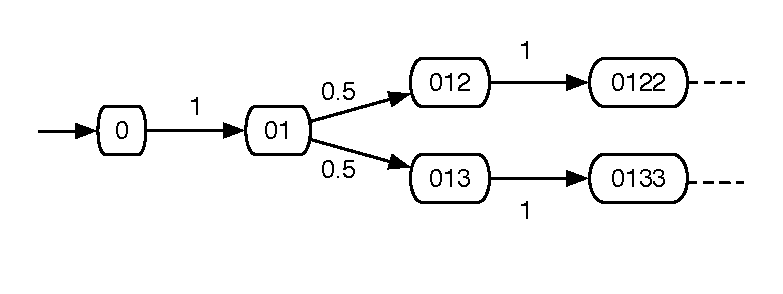
\includegraphics[width=.7\textwidth]{Images/scheduler}
	\end{center}
	\caption{Esempio di \acs{dtmc} derivata dalla \acs{mdp} di figura \ref{fig:mdp:esempio} tramite lo scheduler $\Sigma_1$}
	\label{fig:mdp:scheduler}
\end{figure}
La misura di probabilità definita per le \ac{dtmc} può quindi essere utilizzata per una \ac{dtmc} derivata da una \ac{mdp} tramite uno scheduler. Dato che l'utilizzo di un singolo scheduler risulta eccessivamente restrittivo possiamo generalizzarla per ricercare la massima o la minima probabilità su tutti i possibili scheduler.
